%--- Chapter 2 ----------------------------------------------------------------% 
\chapter{Linear System Solution Methods} \label{LS} 
This chapter presents the popular approaches used for solving linear systems, namely, 
direct and iterative solver techniques. %Section~\ref{LS} introduces linear systems and sections~\ref{DirectSolvers} and ~\ref{IterativeSolvers}
% describe these two most commonly used solving techniques. 
There are mainly two
classes of linear systems-- sparse and dense. The linear systems with majority of
the matrix elements as zero are known as sparse linear systems. The systems with most
of the elements as non-zero are referred to as dense systems. A common
approach of storing sparse matrices involves storing only the non-zero elements, along
with their row and column indexes. For dense systems, all elements need to be
stored, including the zero elements. Problems from various application evolve continuously in time, and can be well represented by large sparse linear systems. Therefore, in this dissertation the main focus is on sparse linear systems.

This chapter presents the two main categories of solvers: direct and iterative, and describes some popular solver techniques which include (1) single-method solver schemes, where only one solver is applied for solving the system, (2) multi-method solver schemes, where more than one solvers are used during different solve stages. 

\section{Motivation}
The solution of large sparse linear systems of the form $Ax = b$, where $A = [a_{ij} ]$ is an $n \times n$ matrix and $b$ is a given right-hand-side vector, is an elementary problem in scientific computing. Advancements in domains such as multi-physics, aerodynamics and others, where the problems can be formulated as partial differential equations, rely heavily on the efficient solution of the linear systems. Frequently, the total time in such formulations is predominated by the time taken to solve the linear systems.

\begin{figure}
\begin{center}
 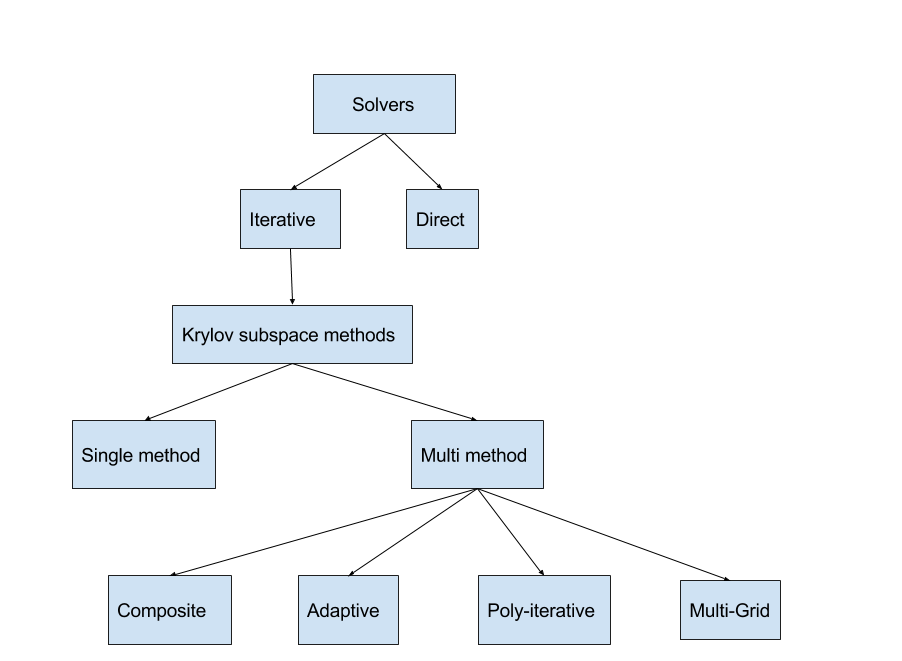
\includegraphics[width=0.95\linewidth]{figures/solver.png}
\end{center}
 \caption{Solver hierarchy showing the different solving strategies.}
 \label{fig:solver}
\end{figure}

The general strategy of solving a sparse linear system of the form $Ax = b$, 
involves transforming the system, $A$ into a similar system which has the same solution, $x$ 
and that is easier to solve. The process of transforming the system into a new system with a reduced condition number, is referred to as preconditioning~\cite{misc3}. Preconditioning is achieved by combining a solver method with a preconditioner. One such transformation 
is pre-multiplying the linear system ($A$) with a non-singular matrix, denoted by $P$. In other words, multiplying 
the left-hand side and the right-hand side with a non-singular matrix. The preconditioning process leaves the solution of the system unaffected. 

There are two popular techniques of solving the systems, namely, direct and iterative solving strategies. Direct solvers have high numerical accuracy and work even for sparse matrices with irregular patterns. Iterative solvers use an initial guess to get an approximation of the solution. For a given approximation solution $x_{k-1}$, the solution, $x_{k}$, at the next iteration is expected to be better. Iterative solvers keep updating the solution until it gets close enough to the actual solution. Figure~\ref{fig:solver} shows the hierarchy of the sparse linear solvers, some of which are discussed in detail in the later sections.

\section{Direct Solvers} \label{DirectSolvers}
For linear systems $Ax=b$, where $A$ is the coefficient matrix, $x$ is the unknown vector and $b$ is the right hand side vector, direct solvers ~\cite{direct1, direct2} provide an exact solution, $x = A^{-1}b$ for the linear system and are more robust than the second category of solvers: iterative solvers. Direct solvers are preferred for small matrices and in cases where an exact solution is required. However, they are less desirable for very large matrices because of their high costs. We focus on sparse matrices for our research and for such matrices, direct solvers may not necessarily generate a solution. This is because the memory requirement for direct solvers can be huge, as direct solvers need the entire matrix to be in memory. For sparse matrices, most of the elements are zero, therefore storing the entire matrix is very expensive. This section describes some of the most commonly used direct solvers.

\subsection{LU Factorization}
For a $n \times n$ matrix $A$, LU factorization factors the original matrix $A$ into the product of the lower triangle of the matrix, represented by $L$ and the upper triangle of the matrix, represented by $U$. In other words, the factorization can be shown by the equation: $A = LU$ where $A$ is the original matrix, $L$ is the lower triangle and $U$ is the upper triangle. A $n \times n$ square matrix $L=(l_{ij})$ is said to be the lower triangular if $l_{ij} = 0$ for $i$ \textless $j$, such that all elements above the diagonal are zero. A $n \times n$ square matrix $U = (u_{ij})$ is considered to be the upper triangle if $u_{ij}$ = 0 for $i$ \textgreater $j$ such that all elements below the diagonal are zero. The factorization can be represented by the following equation: 

\begin{gather} %
\begin{pmatrix}
A_{11} & A_{12} & A_{13} \\
A_{21} & A_{22} & A_{23} \\
A_{31} & A_{32} & A_{33} \\
\end{pmatrix} 
=
\begin{pmatrix}
L_{11} & &  \\
L_{21} & L_{22} &  \\
L_{31} & L_{32} & L_{33} \\
\end{pmatrix}
.
\begin{pmatrix}
U_{11} & U_{12} & U_{13} \\
& U_{22} & U_{23} \\
&  & U_{33} \\
\end{pmatrix}
\end{gather}

The LU Factorization of $A = (a_{ij})$ can be given as the product of the matrices $L$ and $U$. The matrix $L$ should have only ones on the diagonal. The matrices $L$ and $U$ are obtained by applying various row operations to make all the elements below the diagonal and all the elements above the diagonal as zero respectively. The next step involves applying forward and backward substitution to get the solution and the total solution time is dominated by the decomposition of $A$ into matrices $L$ and $U$, which can be given as $O(1/3n)^3$.

Forward substitution for lower triangular system can be given as follows: \\
\begin{center}
$x_{1} = b_{1}/a_{11}$ \\
$x_{i} = \lbrack b_{i} - \sum_{j=1}^{i-1} a_{ij} x_{u} \rbrack / a_{ii}$, where $i = 2, \ldots, n$

Backward substitution for upper triangular system can be given as follows:
\\
$x_{n} = b_{n}/a_{nn}$ \\
$x_{i} = \lbrack b_{i} - \sum_{j=i+1}^{n} a_{ij} x_{j} \rbrack / a_{ii}$, where $i = n-1, \ldots, 1$
\end{center}

LU Factorization technique leads to a unique and robust solution; however the disadvantage is that if the diagonal elements are zero in the start or in any of the intermediary stages, LU Factorization will fail. Also, the memory requirement is large because of fill ins introduced during factorization. This is because in the process of filling, zeros are converted to non-zeros which increases the overall memory requirement. 

\subsection{Cholesky Method}
The Cholesky method is a popular direct method for symmetric positive definite matrices, and the factorization can be shown by the equation:
$A = LL^{T}$, where $L$ is a lower triangle matrix with positive entries on its diagonal. The factorization is shown in the set of equations shown below:

\begin {align*}
 A &= 
    \begin{bmatrix}
     a_{11}       & a_{21} & a_{31} \\
     a_{21}       & a_{22} & a_{32} \\
     a_{31}       & a_{32} & a_{33} 
    \end{bmatrix} \\
&= 
    \begin{bmatrix}
     l_{11}       & 0 & 0 \\
     l_{21}       & l_{22} & 0 \\
     l_{31}       & l_{32} & l_{33} 
    \end{bmatrix}
       . 
    \begin{bmatrix}
     l_{11}       & l_{21} & l_{31} \\
     0            & l_{22} & l_{32} \\
     0            & 0      & l_{33} 
    \end{bmatrix}    
    = LL^T \\
&= 
    \begin{bmatrix}
     l_{11}^2           & l_{21} l_{11}      & l_{31}l_{11} \\
     l_{21} l_{11}      & l_{21}^2 l_{22}^2  & l_{31}l_{21} + l_{32}l_{2} \\
     l_{31} l_{11}      & l_{31}l_{21} + l_{32}l_{22}      & l_{31}^2 +  l_{32}^2 + l_{33}^2
    \end{bmatrix}
\end {align*}

New nonzero entries that appear in $A$ are called fill-in. The system can be solved by computing $A = LL^T$, followed by solving $Ly=b$, and later solving $L^Tx = y$. This method involves computing square roots of some of the elements, such as the first element in the first row. Cholesky method is very popular for its efficiency and stability when solving symmetric linear systems, for the following reasons. Cholesky only requires the lower triangle of the matrix to be stored, so the upper triangle need not be stored at any point in time. It 
requires only $(n^3)/6$ multiplications and a similar number of additions. On comparison, the storage requirement of Cholesky Method is half of the storage requirement of the operations required by other direct methods for non-symmetric systems, such as LU Factorization technique. Computing square roots requires positive entries, which ensures that the algorithm is well defined. In addition, Cholesky method does not require pivoting of any form for stability purposes. In contrast to LU decomposition, Cholesky is more efficient with its time complexity better by a factor of 2; that is, $O (1/3n)^3.$ The space complexity of this method is $O (n^2)$.\\

Cholesky method can be used for problems other than positive definite with a variation (the original Cholesky method fails if the problem involves negative values, as it requires taking square root of a negative element).
This problem can be avoided by using a variant of the Cholesky method, which factors the system as follows: $LDL^{T}$ factorization, where $D$ is the diagonal matrix of the squares of the diagonal entries. This ensures that the variant does not require square roots of any elements. The variant is represented as follows: 

\[
\begin{bmatrix}
    I     & A \\
    A^{T} & 0 
\end{bmatrix}
\cdot
\begin{bmatrix}
    r \\
    x 
\end{bmatrix}
=
\begin{bmatrix}
    b \\
    0 \\
\end{bmatrix}
\]


The matrix above is symmetric, positive definite which can be solved with this factorization. 

\subsection{QR Factorization}
LU factorization and the Cholesky method are based on Gaussian elimination, whereas QR factorization is an orthogonalization method. Some problems cannot be solved with Gaussian elimination, as it does not preserve the Euclidean norm, which therefore does not preserve the solution to the problem. In such situations QR Factorization is applicable. In QR Factorization~\cite{qr}, the matrix is factorized into the product of two matrices: $Q$, the orthogonal matrix, and $R$, the upper triangular matrix; i.e.,$A = QR$. The orthogonal matrix is a matrix such that the product of the orthogonal matrix and its transpose give the identity matrix, 
\begin{center}
$Q^{T}Q = I$ and $Q^{-1} = Q^{T}$. 


$A = QR$ where $R = Q^{T}A$

\end{center}

Now instead of solving $Ax = b$, the equation $Qx=b$ is solved by simply computing $Rx = Q^{T}b$. QR factorization is one of the simpler methods which converts the problem into a triangular problem that is easier to be solved by forward or backward substitution. Similar to Gaussian elimination methods, QR Factorization method also introduces zeros in order to make the problem in the Upper Triangular format. QR Factorization can be computed by many ways, such as plane rotation, Householder transformation and Givens rotation. One popular way is using Gram-Schmidt orthogonalization, which is explained in detail below. There are three main steps of the QR factorization: 
\begin{enumerate}
     \item Find the orthogonal basis for the problem using Gram-Schmidt method: It orthonormalizes a set of vectors in an inner product space. It takes $a_1,a_2,\ldots, a_k$ and generates an orthogonal set $u_1,u_2,\ldots, u_k$ where $a_k$ are the columns of the original matrix, $A$ . The orthogonal basis is computed by the formula shown below:
     \begin{center}
   $u_k = a_k - \sum_{j=1}^{k-1}$ proj\_u\_{j} $a_k$
     \end{center}
     
     \item Convert the orthogonal basis into orthonormal basis: This conversion is done to make them of uniform length. The orthonormal basis is computed as follows: 
     \begin{center}
     $e_k = u_k / ||a_k||$ 
     \end{center}
     Here $e_k$ is the normalized vector and $||a_k||$ is the length of vector $a$.
     
     \item Perform the QR factorization: Once the first two steps have been performed, they will generate $Q$, which is the normalized vector  $e_k$ obtained in Step 2. $R$ is obtained by applying the formula $R = Q^T A$. 
\end{enumerate}

Note that this method requires separate storage for $A$, $Q$ and $R$ matrices because $A$ is used for the inner loop calculations and hence cannot be discarded. The space complexity of this method is $ O (n^2)$ and the time complexity is $ O (4/3 n^3)$. Therefore, orthogonalization methods are more expensive than Gaussian elimination methods, for instance Cholesky method. Although Modified Gram-Schmidt Method can be applied to address the high storage requirement by making $A$ and $Q$ share the same storage. 

\subsection{Frontal Solver Method}
Frontal solver method is used for solving sparse linear systems which are symmetric and positive-definite banded. They are very popular in finite element analysis. It is a slight improvement of the Gaussian elimination and performs better by eliminating more finite elements. Each finite element is associated with some variables and vice versa. This method declares a frontal matrix, which is a dense square sub-matrix, in which all the operations are performed. It starts eliminating finite elements and moves downwards element by element, in a diagonal fashion. It assembles the finite elements (based on an order defined prior to the assembly) then eliminates and updates variables and then again does the assembly. This alternate cycle keeps going till the frontal matrix gets filled. At this stage, the frontal matrix consumes the maximum memory, and from here on, the frontal matrix does not grow in size. Once the frontal matrix is full, a partial factorization is applied on the frontal matrix and elimination is performed. The elements that are fully-summed are eliminated and all the other elements are updated. A variable is said to be fully-summed whenever the last equation in which it occurs is assembled. Those elements that are selected for elimination are removed from the frontal matrix and placed elsewhere. This is then followed by assembly of the new finite elements, which earlier could not be assembled because the frontal matrix had got full. This process continues till all the elements have not been assembled and all variables have been eliminated. The next step is to solve the linear system, using forward and backward substitution.

\section{Iterative Solvers}\label{IterativeSolvers}
Iterative solvers provide an approximation of the solution as the exact solution might either be too expensive to compute. Iterative solvers start with an initial guess and generate successive approximations to the solution. In cases of large linear systems, iterative methods are more useful. The traditional approach of solving large sparse linear systems involves using a solver combined with a preconditioner. There are many solver techniques that have been in existence for solving large sparse linear systems of the form $Ax = b$ where $A$ is the sparse matrix, $x$ is the solution vector and $b$ is the right-hand side vector (known vector). The residual norm can be given as $Ax - b$. The aim with iterative solvers is to reduce the residual norm as much as possible. 

One of the popular classes of iterative numerical solvers is the Krylov subspace methods. Krylov subspace methods start with an initial guess and generate a sequence of approximate solutions, which tend to improve with the progression of iterations. Krylov methods form a sequence, called the Krylov sequence shown below: 

${K}_{k}(A,b)= span\{b_0,Ab_0,A^{2}b_0,\ldots,A^{k-1}b_0\}$

Here $A$ is a $n \times n$ matrix, $b$ is a vector of dimension $n$, $k$ is the order of the subspace, $b_0$ is an initial vector of successive matrix power times the initial residual (the Krylov sequence). The subspace is the successive powers of the matrix $A$ starting from $0$ to $k-1$ applied to the residual form. The approximations to the solution are then formed by minimizing the residual over the subspace formed. They are considered to be desirable for solving linear and non-linear systems because of their efficiency and reliability. 

%PETSc
This dissertation focuses on using solvers and preconditioners offered by PETSc~\cite{petsc}. Portable Extensible Toolkit for Scientific Computing (PETSc) is a widely used toolkit for linear systems, developed at Argonne National Laboratory. PETSc is a collection of data structures and functions for the scalable (parallel) solution of scientific applications and offers solver techniques and preconditioners for linear and non-linear equations. PETSc can run on different architectures, various operating systems and is portable to any parallel system that supports MPI. PETSc is widely used for modeling small-scale and large-scale applications as it is highly efficient. PETSc offers scalable solutions for scientific applications ranging from brain surgery~\cite{petscapp1}, cancer treatment~\cite{petscapp2}, earthquakes~\cite{petscapp3}, ocean dynamics~\cite{petscapp4}, among many others. Figure~\ref{fig:petscFlow} shows the flow control for a PETSc application. The rest of the section describes some of the most popular Krylov subspace methods for symmetric and non-symmetric matrices offered by PETSc and used throughout this research. 

\begin{figure}
\begin{center}
 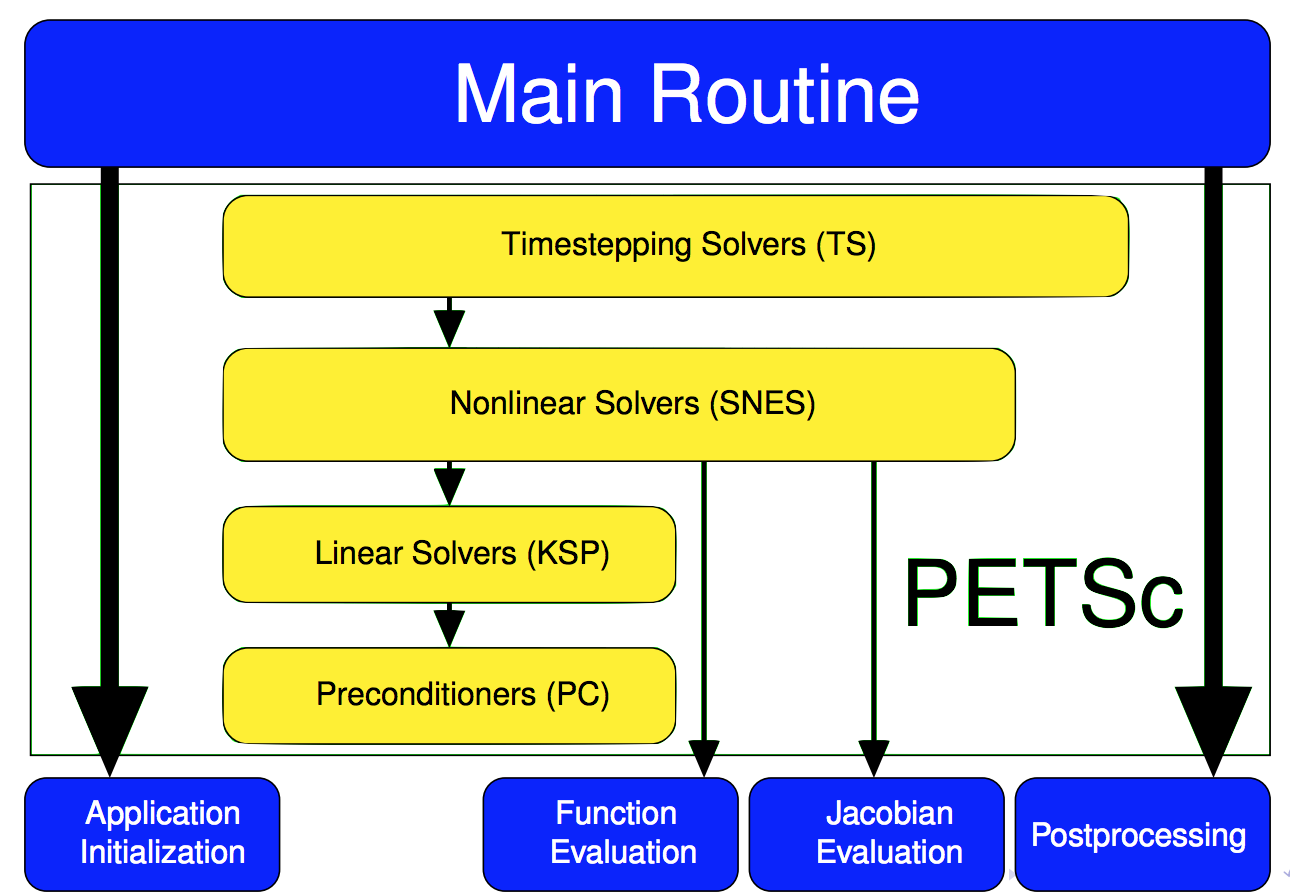
\includegraphics[width=0.7\linewidth]{figures/FlowControlForPETScApplication.png}
\end{center}
\caption{Flow control for a PETSc application. [Source: PETSc tutorial https://www.mcs.anl.gov/petsc/documentation/tutorials]\label{fig:petscFlow}}
\end{figure}

\subsection{Conjugate Gradient Method}
Conjugate Gradient (CG) method ~\cite{cg1,cg2,cg3} is applicable for symmetric linear systems. CG starts with an initial guess of the
solution, an initial residual and an initial search direction. It looks for approximate solutions at each step within its Krylov subspace as shown below: 
\begin{center}
${K}_{k} = span\{b,Ab,A^{2}b,\ldots,A^{k-1}b\}$ for $k \geq 1$
\end{center}
It finds a series of gradients (conjugate vectors) $x^{0}, x^{1}, \ldots$ until the point where the gradient gets sufficiently close to the solution. The gradients are given by the equation shown below: 
\begin{center}
$x_{k+1} = x_{k} + \alpha_k s_k$
\end{center}  
Here $\alpha_k$ is a scalar determining the step length and $ s_k$ is the search direction. The minimum over $\alpha $ occurs when the residual is orthogonal to the search direction. Each iteration requires only one matrix-vector multiplication. They are also the gradients of a quadratic function shown below, the minimization of which is the same as solving the system:
\begin{center}
$\phi(x) = 1/2 x^{T}Ax - x^{T} b $.
\end{center}
Initially, $s_0 = r_0 = b - ax_0$, and the residual is updated in the following way:
\begin{center}
$r_{k+1} = b - Ax_{k+1} = r_k - \alpha_k A s_k$.
\end{center}
The storage requirement of Conjugate Gradient is low, as it only needs to store vectors $x$, $r$ and $s$, and they can be overwritten after each iteration. The convergence rate depends on the square root of the condition number. It is an extremely popular solver technique for symmetric, positive definite matrices. Conjugate Gradient method became the ground for many other solver methods, which were variants of Conjugate Gradient, such as BiConjugate Gradient method, BiConjugate Gradient Stabilized method, Conjugate Gradient Squared and Improved Stabilized version of BiConjugate Gradient Squared method (some of which are described in the following section).

\subsection{Variants of Conjugate Gradient Method}
Biconjugate gradient(BiCG) method ~\cite{bicg1} is implemented, similar to running the conjugate gradient on the normal equations except that it maintains a second Krylov subspace. Therefore, BiCG has more matrix-vector multiplications and dot products than CG method. It solves the system $Ax = b$ as well as $A^Tx^* = b^*.$ The advantage of BiCG over CG is that it can solve more variety of matrices, like symmetric positive definite matrices, non-symmetric matrices.

Biconjugate gradient stabilized method (BiCGStab) ~\cite{bicgstab}, is an iterative Krylov subspace method for the numerical solution of non-symmetric linear systems which is a variant of the bi-conjugate gradient method (BiCG). It computes $i |->Q_i(A)P_i(A)r^{(0)}$ where $Q$ is an $ith$ degree polynomial describing a steepest descent update. It has a faster convergence than the original method as well as other variants such as the conjugate gradient squared method (CGS). This method involves two matrix-vector products more than the BiCG method. The advantage is, it avoids the irregular convergence patterns, which are observed in other variants of CG method. 

Improved Stabilized version of BiConjugate Gradient Stabilized((IBiCGStab) method ~\cite{ibcgs} is another variant of CG method series. It is an improved stabilized version of BiConjugate Gradient Stabilized method. This method attempts to reduce the computational cost of the BiCGStab method. 

Conjugate-Gradient Squared(CGS) ~\cite{cgs} method is a variant of BiCG algorithm, the difference being that this method does not involve adjoint matrix-vector multiplications and the expected convergence rate is expected to be better than BiCG method. Transpose-Free Quasi-Minimal Residual Method (TFQMR) ~\cite{tfqmr} is a quasi-minimal residual version of CGS method. It retains the desirable convergence features of CGS and corrects its erratic behavior.

\subsection{Chebyshev Method}
Chebyshev method ~\cite{chebyshev} is a solver method that can be used for either symmetric or non-symmetric matrices. It is a variant of CG method except that Chebyshev iteration method avoids computing inner products, removing the operations with the inner products, unlike GMRES and CG methods. This method needs knowledge about the spectrum of the matrix $A$, which is given by the lower estimate of the lower eigen value and the upper estimate of the upper eigen value. Once the ellipse containing the eigen values is known, the iteration parameters become known as well. Two scalar values, $c$, $d$ are needed to define the ellipses such that they have common center $d>0$ and foci $d+c$ and $d-c$ which contain the ellipse that surrounds the spectrum. 
\subsection{Quasi-Minimal Residual Method}
QMR ~\cite{qmr} is a quasi-minimal residual method for non-Hermitian linear systems. It looks ahead to generate vectors for the Krylov subspace. QMR has smooth convergence curves and good numerical properties. When compared to BiCG, QMR is less prone to breakdowns and is more stable. TCQMR ~\cite{overview} is a variant of quasi-minimal residual provided by Tony Chan. 

\subsection{GMRES Method}
Another category of solvers includes Generalized minimal residual (GMRES) method and variants of it, such as, Flexible GMRES and LGMRES. GMRES method ~\cite{gmres1, gmres2} and its variants are used for non-symmetric matrices. It approximates the solution by the vector in a Krylov subspace with minimal residual. The Arnoldi iteration is used to find this vector. FGMRES method ~\cite{fgmres1,fgmres2} is a generalization of GMRES that allows larger flexibility in the choice of solution subspace
than GMRES method allowing any iterative method to be used as a preconditioner. LGMRES ~\cite{lgmres,lgmres2} augments the standard GMRES approximation space with approximations
to the error from previous restart cycles. This method supersedes the original method by accelerating the convergence of restarted GMRES. It is more like CG with polynomial preconditioning.

\subsection{LSQR}
LSQR ~\cite{lsqr1,lsqr2} is an algorithm for sparse linear equations and sparse least squares. It is one of the oldest methods in the history of iterative solvers. The algorithm is based on generating a sequence of approximations in a manner that the residual norm decreases monotonically. Some of the advantages of this solver are high efficiency, and high convergence speed for a variety of linear systems. The memory requirement for these systems scale with the dimensions of the matrix and work well in parallel setups. It has been observed in the past that this method is more reliable than the other solver techniques and hence is popular in many domains, for instance, it has been a common choice for seismic tomography since many years in the past. 

\subsection{ Jacobi Method}
Jacobi method is a solver technique in which the original matrix $A$ is split into two matrices, say, $S$ and $T$, such that, $A = S + T$, where $S$ is the diagonal matrix of $A$ and $T$ is the original matrix with the diagonal matrix removed, leaving the remainder, shown as, 
\begin{center}
$S = diag(A) = D_{A}$ and $T = A - D_{A}$
\end{center}

Once the diagonal matrix is obtained and the original matrix is split into S and T matrices, an update is performed according to the following update rule:
\begin{center}
$Ax = b,$ $A = S+T$ and $S = D_{A}$

$(S + T)x = b$

$(D_{A} + A-D_{A})x = b$ \\
For each iteration, to obtain the next successive solution the below rule is used.
$x^{(k+1)}=D^{-1}_{A}(b -(A-D_{A}) x^{k})$
\end{center}

This method has a simple formulation; given an initial guess, let us say $x^{0}$, for the solution, we can obtain $x^{k}$ so that
\begin{center}
$x^{k}_{i} = \lbrack b_{i} - \sum_{j = 1, j \neq i}^{n} a_{ij}x^{k-1}_{j} \rbrack / a_{ii}$. 
\end{center}
This method requires double storage for the solution vector, because all the old values are needed for the sweep process to get the new values; so at a given time, it stores the old and the new values of $x$ shown in equation above, and that causes the double storage demand. In addition, the Jacobi method is extremely slow, because in each iteration, it solves every variable locally with respect to other variables. So each variable is solved once in each iteration. The rate of convergence is $ (\pi^{2} /log 10) s^2 /2 $.
Here $s$ is the mesh size, which is $1/n+1$, for an $n \times n$ matrix.
This is a solver method that is common for diagonally dominant system. One of the reasons it is very popular is because it is highly parallelizable.

\subsection{ Gauss-Seidel Method}
This method takes advantage of the fact that the latest information obtained in the first iteration can be used in the subsequent iterations. This also increases the convergence of the solver. However, the disadvantage of that is, with this scheme although it allows using the latest information obtained during the present iteration to be used in the upcoming iterations, it looses the resource of parallelism that Jacobi had. 
$x^{k}_{i} = \lbrack b_{i} - \sum_{j = 1}^{i-1} a_{ij}x^{k-1}_{j} - \sum_{j = i+1}^{n} a_{ij}x^k_{j} \rbrack / a_{ii}$. 

\subsection{ Successive Over-Relaxation Method}
Successive Over-Relaxation (SOR)~\cite{sor} is an improvement of the Gauss-Seidel method. Although the Gauss-Seidel Method is faster than the Jacobi Method, it is still slow. SOR achieves an improvement over the convergence rate of the Gauss-Seidel method by reducing the norm of the residual vector. 
Starting with $x^{k}_{i}$, $x^{k+1}_{i}$ is computed the way Gauss-Seidel method would compute, shown by the equation below:
\begin{center}
$x^{k+1}_{i} = (b_{i} - \sum_{j = 1}^{i-1} a_{ij}x^{k}_{j} - \sum_{j = i+1}^{n} a_{ij}x^{k+1}_{j}) / a_{ii}$. 
\end{center}

\begin{center}
Also written as $x^{k+1}_{i} = x^{k}_{i} + r^{k+1}_{ii} a_{ii}$ where $r$ is the residual vector.
\end{center}
SOR uses the next iteration as a search direction with a fixed relaxation parameter, called $\omega$. So the above equation changes to 
\begin{center}
$x^{k+1}_{i} = x^{k}_{i} + \omega r^{k+1}_{ii} a_{ii}$ 
\end{center}
That is, $x^{k+1}_{i}$ is computed by taking a weighted average of the present iteration and the next Gauss-Seidel iteration. The value of $\omega$, if taken as one, gives the Gauss-Seidel method. A value less than one gives under-relaxation, which takes more time to converge than the Gauss-Seidel method. A value in between one and two gives over-relaxation and gives a faster convergence rate than the Gauss-Seidel method.
The rate of convergence for SOR is much improved from Jacobi and Gauss-Seidel. The convergence rate is $ (2 \pi /log 10) s  $; where $s$ is the mesh size which is $1/n+1$, for an $n \times n$ matrix.

\section{Single-Method Solver Systems}
In this approach, only one method is used to solve the given linear system, as shown in ~\cite{direct1, lsqr2, lsqr1, cg1, gmres1, bicgstab, chebyshev, fgmres1, fgmres2, bicg1}. The choice of solver is made, based on the characteristics of the problem. For instance, for symmetric positive definite matrix, Conjugate Gradient is a suitable choice. For non-symmetric matrices, BiConjugate Gradient becomes more preferable. For sparse least squares problems, ill-conditioned problems, Sparse QR factorization is a popular choice. For well-conditioned problems, Cholesky factorization can be used. 

If the method applied to solve the system fails, there is no other solving technique applied to the problem. Depending on the problem, either direct or iterative methods can be used in this approach. Direct solvers generate a solution by performing finite number of operation. Direct solvers get very close to the exact solution. Iterative solvers start with an initial guess and update the solution in every iteration. The iterations are continued until an acceptable approximation, which is defined by the tolerance defined by the user, has been obtained. Hence iterative solvers provide approximations of the solutions, that can be used accordingly for small and large problems. As the problems tend to grow bigger, iterative solvers become a preferable choice. However, in some large-scale applications, direct solvers are used because of non-familiarity with the iterative solvers. 

A single-solver scheme is useful in situations where the solver technique to be used is established. One of the disadvantaged of using a single solver is that, the numerical properties of a system can change during the course of the nonlinear iterations and the single-solver does not take that into consideration.

On the other hand, using multi-method schemes, makes it complex as the number of decisions to be made are more, for instance, which all base methods to be used, when should a new solver be applied, which solver should be applied next, when do we eliminate a solver from the list of base methods, etc. 

\section{Multi-method Solver Systems} 
In a single solver scheme, the choice of the solver method is made by experts or resources available for a selection. However, in many cases there is often no single solver that is consistently better, even for problems from a single application domain. There is also no guarantee that the solver technique used to solve the system will eventually converge. These challenges generated the idea of a solving strategy that involved more than one solver algorithm. The earliest work ~\cite{earliest1,earliest2} which suggested that the efficiency of a system is expected to improve with polyalgorithm solvers, used three basic solvers. The work presented in ~\cite{earliest2} provides the design details of a polyalgorithm for automated solution of the equation $F(x) = 0$. The challenges for the work include the small number of problems available for solving. In addition, the system did not find all the roots for the equation mentioned above and for some of the roots it found out, they were questionable.

The second approach involves using multiple solvers (a composite of suitable solvers)~\cite{multimethod1,multimethod2,arms,dynamic}, instead of a single solver. If two or more solvers are used instead of one, the chances of getting to a solution increase. Further, there are different techniques of using multiple solvers for solving sparse linear systems: composite solvers, adaptive solvers and poly-iterative solvers. These are discussed in detail later in this section. The first technique has the solvers arranged in a sequence. It picks the first solver in the order and tries to solve the system; if this solver fails, it uses the next solver in the list. The second technique uses only one solver, but which solver would be used is decided dynamically. The third technique solves the system with multiple solvers simultaneously. As soon as a solver gets to a solution, the computation by the rest of the solvers is terminated.

In this section, we talk about different types of multi-method solvers approaches namely composite solvers, poly-iterative solvers and adaptive solvers. Multi-method linear systems include a variety of techniques like composite solvers, iterative solvers and adaptive solvers. Below are the papers that cover the variety of multi-method solver techniques that are popular for use.

\subsection{Composite Solvers}
A composite solver approach is the one in which basic solver methods are sequenced in an ordered fashion ~\cite{composite1,composite2,composite3,composite4,composite5}. The first choice for solving the system is the first solver method in the sequence. If a method fails, then the next method in the sequence is invoked. This continues to happen till the problem is solved successfully. The composite algorithms are developed to have efficient and robust solvers as composites of multiple solver methods. The work ~\cite{composite1} achieves this by using multiple preconditioned iterative methods in sequence to provide a solution. The solution obtained by this strategy is believed to be reliable and have a good performance in parallel. This scheme has been tested in a driven cavity flow application for performance. 

As mentioned in ~\cite{composite5,composite1}, the reliability of a method is given as $r_i$ = 1 - $f_i$, where $f_i$ refers to the failure rate. The run time of the composite scheme depends on the sequence of the solver methods. The worst case time scenario for the composite scheme is when it needs to attempt solving the system with all the solver techniques in the given sequence. This can be given by the sum of the time taken by all the solvers in the sequence, in an attempt to solve the system. The total time can be given as follows: 

$T_\pi = t_{\pi(1)} + f_{\pi(1)}.t_{\pi(2)} + f_{\pi(2)}.t_{\pi(3)} + ....(f_{\pi(1)}... f_{\pi(n-1)}) t_{\pi(n)}. $

To have minimum worst-case running time among all the possible combinations possible, the base methods are arranged in the sequence in the increasing order of their utility ratio, $u_i$ which is given by the ratio $t_i/r_i$. For computing this ratio, $r_i$ is substituted as shown below and using estimates of $t_i$ with some sampling technique: $r_i$ = 1 - $f_i$. This also means that the composite solver technique uses knowledge obtained in the past, which enables using domain-specific knowledge for the selection of solvers. This system maintains the past performance history and allows monitoring system performance.

The solvers are then arranged in the increasing order of their utility ratio, $u_i$. They use a simple sampling technique for the optimal composite by computing this ratio from running all the solver methods in the sequence on a small dataset and obtaining the mean of the time taken per iteration by the solvers and the failure rates.

The software architecture that supports this strategy is shown in Figure~\ref{fig:composite_multimtdarchitecture}. It has the following components: solver proxy, non-linear solvers, linear solvers, ordering agent and application driver. The proxy linear solver method acts as an intermediate between the non-linear solver algorithm and linear algorithm. The proxy, linear solvers and non-linear solvers have the same solver interface to make it easy to use multiple solvers. This proxy interacts with the ordering agent to choose the linear solvers based on the ordering strategy. The proxy is used with Newton-Krylov solver. They use the following four set of base solution methods: (1) GMRES(30), restricted additive Schwarz method (RASM)(1) with Jacobi subdomain solver (2) GMRES(30), RASM(1), with SOR subdomain solver (3) TFQMR, RASM(3) with no-fill ILU subdomain solver and (4) TFQMR, RASM(4) with no- fill ILU subdomain solver. The numbers in brackets denote the degree of overlap. 

\begin{figure}[h]
\begin{center}
 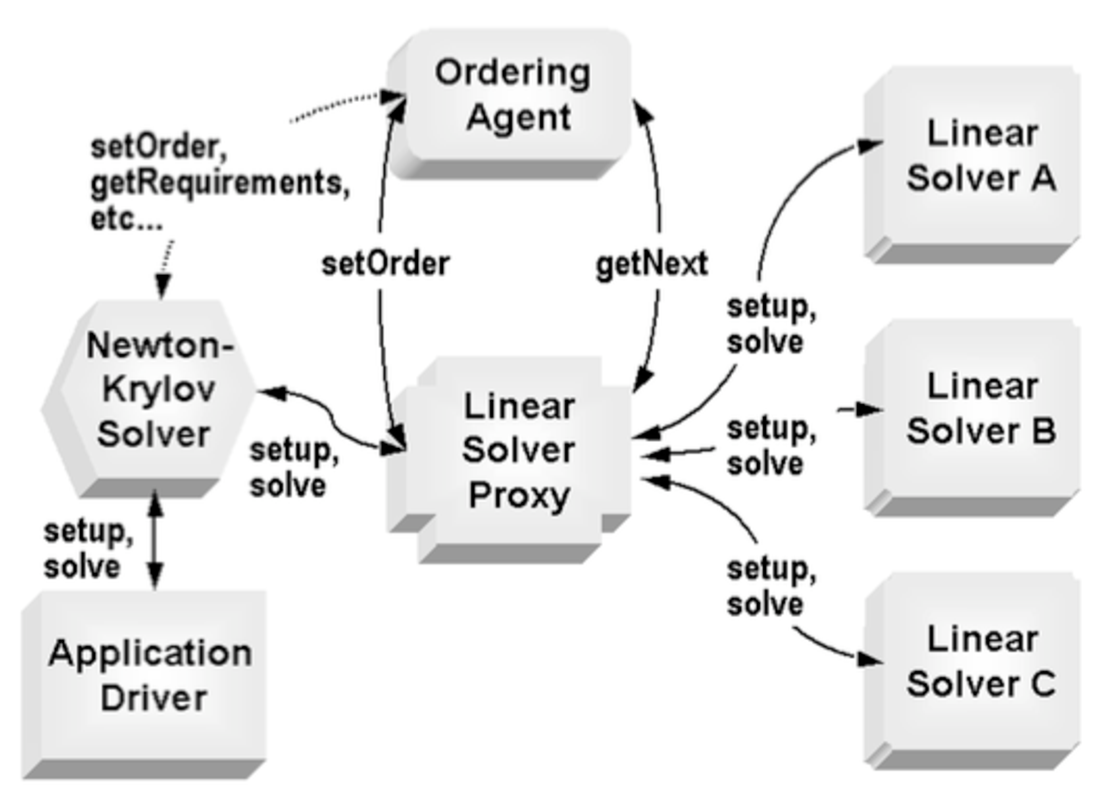
\includegraphics[width=0.7\linewidth]{figures/composite_multimtdarchitecture.pdf}
\end{center}
\caption{Multimethod software architecture.\label{fig:composite_multimtdarchitecture}}
\end{figure}


\subsection{Adaptive Solvers}
In this approach ~\cite{adaptive1,adaptive2,adaptive3,adaptive4,adaptive5} only one solver is used by selecting the most suitable solver dynamically, based on the match of the solver with the characteristics of the linear system under consideration. This technique adapts the solver method during a simulation, based on the changing attributes of the problem. The advantage this approach has over the composite solve approach is that it uses only one base solver for each linear system. 

Numerical properties for a system change at each iteration of solving simulation and so does the choice of the solver and the selection criteria. In ~\cite{adaptive1} linear solvers are selected at each iteration based on the characteristics of the problem emerging at each level and given the nature of the problem at that stage, the decision of the best suited solver is taken at each stage. This strategy applies a different preconditioner during different simulation stages maintaining a low overall time for finding the solution. This was done by the combination criteria for different methods. For instance, if there was a more robust method at one stage, then the other stages had methods that were faster to compensate the time taken by the first method. They used GMRES(10) with a point-block ILU(1) preconditioner. With this approach, the chances of getting a solution are increased, as there are robust methods involved and also the total time for the solution is acceptable as well. The work described in ~\cite{adaptive4} is an extension of the previous work, to solve a more complex parallel application to show that the adaptive poly-algorithmic approach is parallelizable and scalable. They were four linear solvers used: 
\begin{itemize}
    \item GMRES with a block Jacobi preconditioner that with SOR as a subdomain solver, called GMRES-SOR.
    \item Bi-conjugate gradientsquared (BCGS) with a BJ preconditioner and no-fill incomplete factorization (ILU(0)) as a subdomain solver, called BCGS-ILU0.
    \item Flexible GMRES (FGMRES) with a BJ preconditioner with ILU(0) as a subdomain solver, designated as FGMRES-ILU0
    \item FGMRES with a Block Jacobi preconditioner that uses ILU(1) as a subdomain solver, called FGMRES-ILU1.
\end{itemize}

The switch is made on the following two indicators: 
(1) The nonlinear residual norm is calculated and assigned to the following four categories: 
(a) $||f(u)|| \geq 10^{-2}$, (b) $10^{-4} \leq ||f(u)|| < 10^{-2}$, (c)
$10^{-10} \leq ||f(u)|| < 10^{-4} $, and (d) $||f(u)|| < 10^{-10}$
A change in the solver is made when the simulation moves from one category to another and the solver method is moved up or down accordingly. 
(2) Average time per nonlinear iteration:
The base solver methods are arranged in increasing order of their corresponding average time per nonlinear iteration values.

On the other hand, the research ~\cite{adaptive2} has a different approach. It uses statistical data modeling for making the solver choice automatically. They combine different solver techniques with different preconditioners and different parameters as well.

\subsection{Poly-iterative Solvers}
Poly-iterative solver approach uses multiple solvers applied simultaneously to the system so that the chances of getting a solution increase. If one solver fails, one of the other solvers from the system can provide a solution. One of the earliest suggestions made in ~\cite{earliest1} for poly-iterative solver strategy was made in late 1960's. This strategy is based on selecting the solver based on the problem size and the user's specifications about the problem and the accuracy level expected from the system. If no information is specified by the user, then the size is used to pick the solver. If it is a small matrix, with less than 15 rows and 15 columns, the solver chosen is LU decomposition. If LU decomposition method fails, then the solution obtained just before the fail is taken as initial guess for SOR. If SOR method also fails, the user is provided with the summary and prompted for further instructions to solve. The user may lower the accuracy level to accept somewhat less acceptable solution or allow longer computations for solving the systems. 

For problems of large size (considered large in that decade), more than 80 rows and columns, SOR is applied. If this fails, SOR is applied again but this time on the product of matrix transpose and the original matrix. If this strategy fails then the user is asked for further instructions similar to the small matrix scheme. For problems with intermediate size, properties namely bandedness, diagonal nature are investigated and if either of these properties are valid for the problem in consideration, SOR is applied. If that fails, LU decomposition is tried. If that fails as well, then the system relies on the user feedback for accepting lower accuracy level or allowing longer computations.

The work in ~\cite{bombardment} with the poly-iterative approach ~\cite{earliest1,poly1,poly2} mentions the advantages of using a poly-iterative approach in parallel; firstly, having an increased probability of finding a solution. Secondly, increased performance resulting from an efficient matrix-vector product. In addition, once any one of the solver methods has converged, the process can be terminated. This algorithm uses three solver techniques: 1. QMR 2. CGS 3. BiCGSTAB. These methods start computing the inner product, then perform the vector updates and finally a preconditioner solve. All these methods are applied simultaneously and as soon as one of them converges, the iteration is stopped for all other methods. The cost per iteration is the sum of the cost of the three methods. In case if a method fails, it is removed from the iterative scheme. This strategy takes more time than the best method but is preferred as it has a higher probability of finding the solution. The extra time is due to the communication cost involved in this strategy although it may be reduced by making communications global. Another situation in which this method incurs higher cost is when one of the methods is comparatively more expensive than the others and it is not the first method to converge nor it fails. However, this strategy is more beneficial in parallel implementation as this approach aligns the mathematical operations of the solver methods and combines the communication stages to make it more efficient. Figure ~\ref{fig:bombardment} shows the sequence of operations and how the communication is combined. 
\begin{figure}[htp]
\begin{center}
 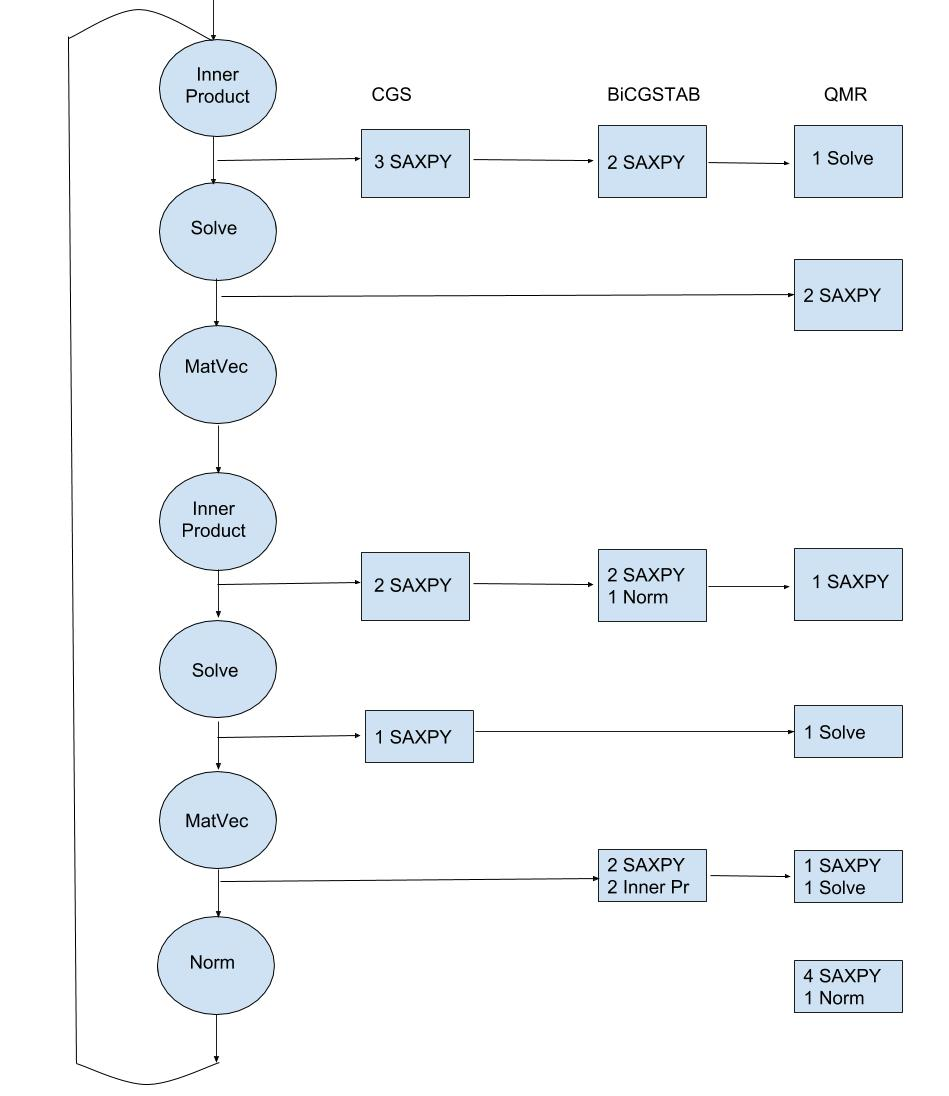
\includegraphics[width=0.7\linewidth]{figures/bombardment.jpg}
\end{center}
 \caption{Sequence of operations.}
 \label{fig:bombardment}
\end{figure}


The work~\cite{poly1} provides methods that can be used for automatic solution of $F(x) = 0 $ where $F(x)$ is the non-linear equation for one variable. It uses three base methods: Secant method, half interval method and descent method.
\begin{enumerate}
\item Secant method: Secant solver is one of the oldest solver methods in the history of numerical analysis. It is a root-finding algorithm that finds roots in succession to get an approximation of the root. This method is an approximation of the Newton's method. The secant method is as follows: 

$x_{n}=x_{n-1}-f(x_{n-1}){\frac {x_{n-1}-x_{n-2}}{f(x_{n-1})-f(x_{n-2})}}={\frac {x_{n-2}f(x_{n-1})-x_{n-1}f(x_{n-2})}{f(x_{n-1})-f(x_{n-2})}}$

\item Half-interval method: This method works in conjunction with the previous method. It applies secant method for a short run for both the intervals; each interval being half of the total time. If none of these secant method work, the point at which the sign changes is classified as a discontinuity. 
\item Descent method: This is descent on the absolute function of the non-linear equation used to alter the location of the root. It is used only when a root is found by the secant method and cannot be used standalone.

\end{enumerate}
\subsection{ Self Adapting Solvers Large-Scale Solver Architecture (SALSA) Solvers}
SALSA ~\cite{salsa} is a self adapting solver technique which has several levels on which the computational choices for the application scientist is automated. The choice of solver technique can be made based on the nature of data and on the efficiency of the available kernels on the architecture under consideration to facilitate tuned high-performance kernels. One of the advantages of this scheme is that it is expected to increase its intelligence gradually. SALSA remembers the results of the runs and learns over time. There are three levels of adaptivity: 
\begin{enumerate}
\item Kernel level: It can be done in one-time installation and is independent of the data given by the user.

\item Network level: Some level of interaction with user data.

\item Algorithm level: At this level, analysis is done dynamically based on the user data.
\end{enumerate}

\subsection{Linear System Analyzer Solvers}
The Linear System Analyzer(LSA) ~\cite{lsa} is a component-based problem-solving environment for large sparse linear systems. The components LSA provides are broadly categorized in four categories: IO, Filter, Solver and Information. IO is for feeding the problem into the system and getting the solution out of the system. The user also feeds various parameters and settings for solving, such as the relaxation for solving, what solver to be used for solving etc. Although this system takes a lot of input from the user apart from the problem to be fed as input, it provides settings to choose default parameters for the various solving techniques and other settings shown on the interface. Figure~\ref{fig:lsa1} shows a sample LSA session. Filter is for providing filtering of data or system manipulation in other words, such as scaling, eliminating entries based on the size etc. Solver is for actually getting the system solved. LSA offers for choices to the users to use for solving. They are as follows:

\begin{enumerate}
\item Banded: A matrix has a banded structure if its rows and columns can be permuted such that the non-zero entries form a diagonal band, more like exhibiting a staircase pattern of overlapping rows. It converts the system to banded structure and solves the system, with the new data structure and uses LINPACK ~\cite{linpack} routines for solving. LINPACK, LINear algebra PACKage is a Fortran package developed in 1970's. It uses BLAS as the underlying routine.
\item Dense: It converts the system into a dense 2D array data structure and then solves it using Lapack ~\cite{lapack} routines.
system to a dense 2D array data structure.
\item SuperLU: SuperLU ~\cite{superlu} is a solver library for getting direct solutions for large, sparse, non-symmetric systems of linear equations.
\item SPLIB: They use preconditioned iterative solvers offered by SPLIB library~\cite{splib}. This library had 13 solvers and 7 preconditioners when this research was performed.
\end{enumerate}


\begin{figure}[htp]
\begin{center}
 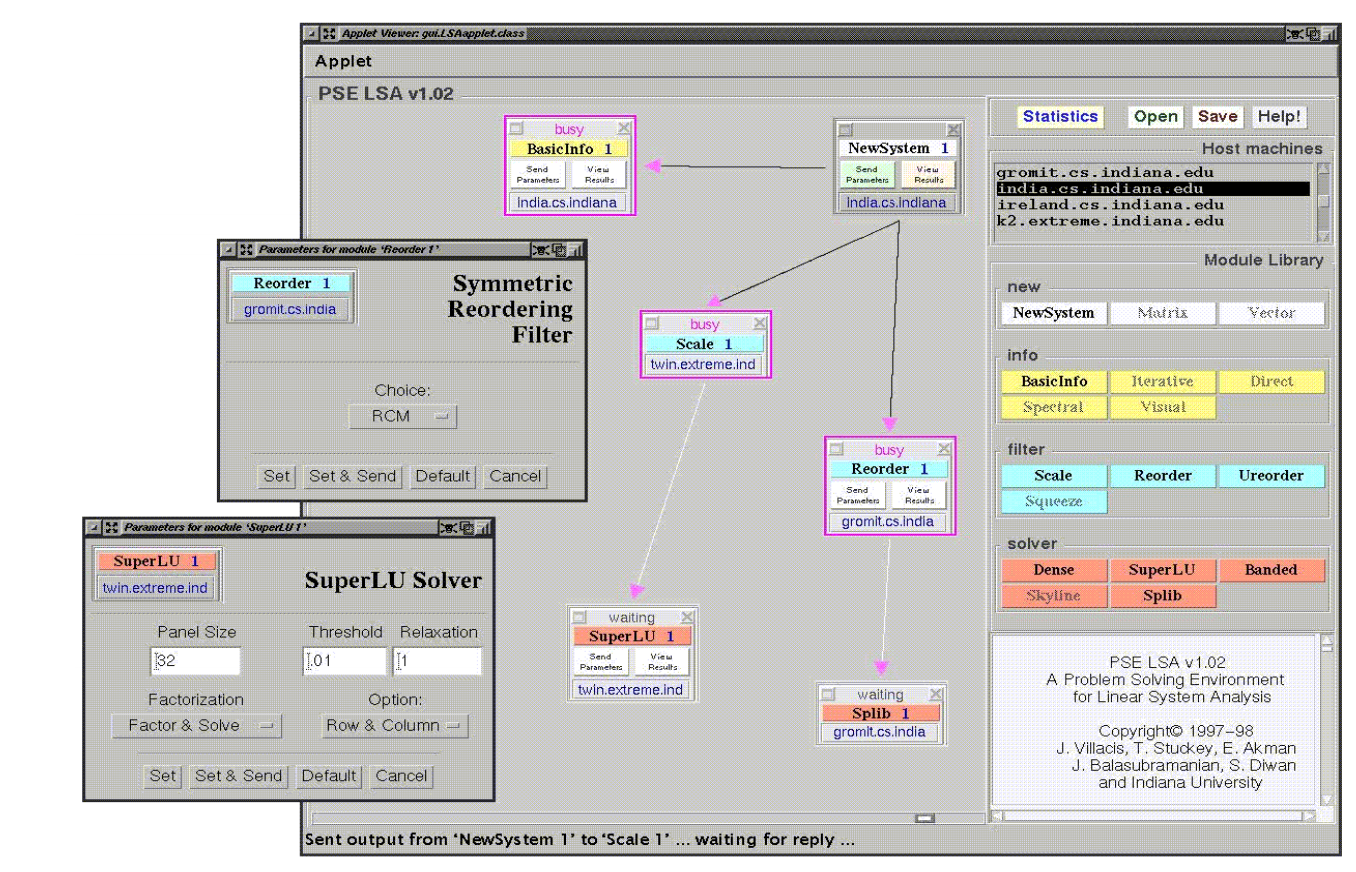
\includegraphics[width=0.9\linewidth]{figures/lsa1.png}
\end{center}
 \caption{Sample LSA Session.}
 \label{fig:lsa1}
\end{figure}

Figure ~\ref{fig:lsa} shows the LSA architecture with its four components namely, user control, manager, communication subsystem, and information subsystem.
This approach provides parallelism between components, which supports solving large problems by simultaneously using the computational resources of multiple machines. This system allows comparisons of different solver methods and support to facilitate practical solution strategies. 

\begin{figure}[htp]
\begin{center}
 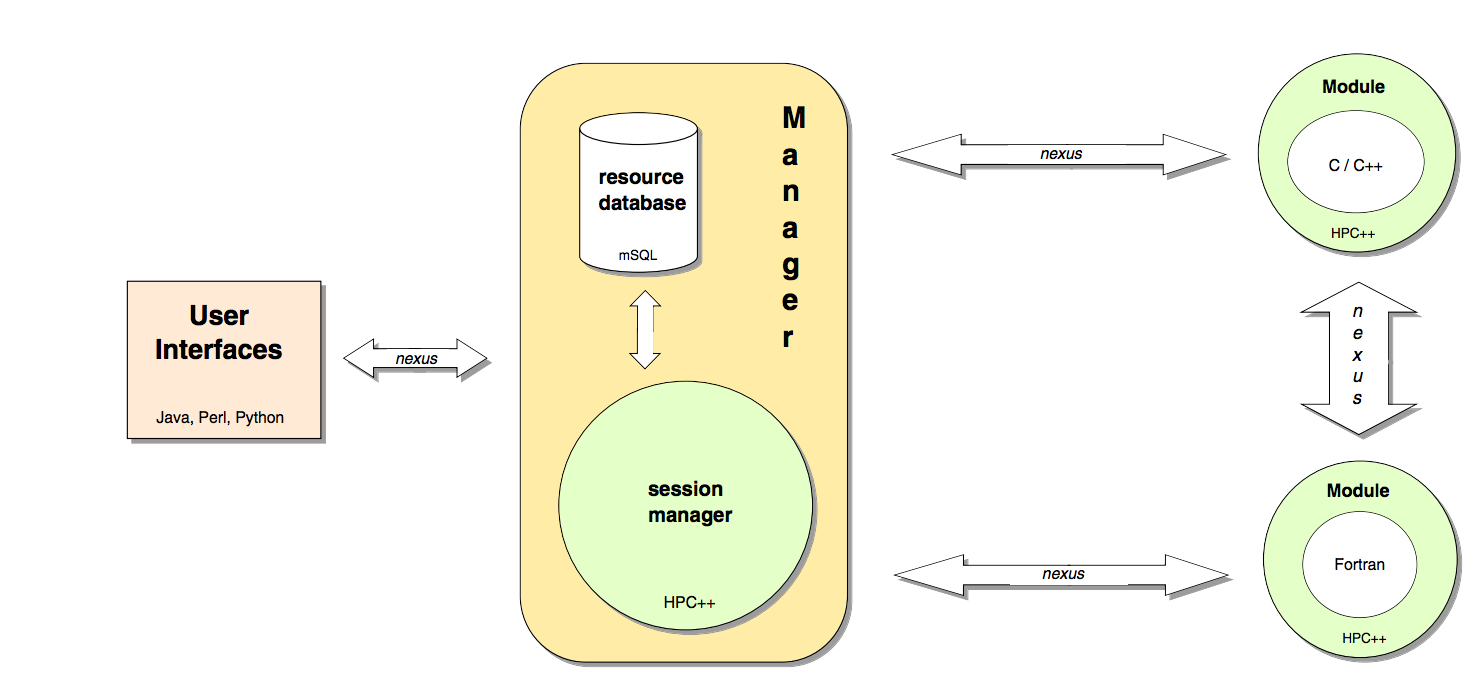
\includegraphics[width=0.9\linewidth]{figures/lsa.png}
\end{center}
 \caption{LSA Architecture.}
 \label{fig:lsa}
\end{figure}


The user control module is a Java interface. A new system is fed as input in the 
first component in the module ``NewSystem''. In the meanwhile, the matrix is scaled and reordered, both simultaneously on different machines. These actions are performed through the user control module, which also has options for choosing parameters for all the modules in the interface. The scaled problem is sent to SuperLU and the reordered version is sent to SPLIB where SuperLU and SPLIB are the two component subinterfaces. LSA has an option of running multiple solvers on a single system in order to compare these techniques and use them for research purposes.

The LSA manager collaborates control and resource management. It establishes a component network to facilitate multiple user control systems with a single LSA session. It also assigns unique identifiers and maintains the database of various machines and components.

The next module is the communication subsystem which is Nexus ~\cite{nexus} which is a cross-platform system for facilitating parallel applications and distributed computing. LSA uses a bunch of libraries for solvers and preconditioners that are written in different programming languages and therefore there needs to be a module that handles this and make it robust as a mixed language system. Nexus provides this bridge between the different languages used in LSA.

The Information subsystem module provides any information that the user may want about the solving process except the undesirable information. The results are shown in the form of a a summary with the performance metrics for that scenario. There is a small description provided, along with the details whether the event was successful or failure or there was a warning. The user is also redirected to more information, in case if he wants more details. 

\subsection{Finite Element Tearing and Interconnecting and its parallel solution algorithm(FETI)}

\begin{figure}[htp]
\begin{center}
 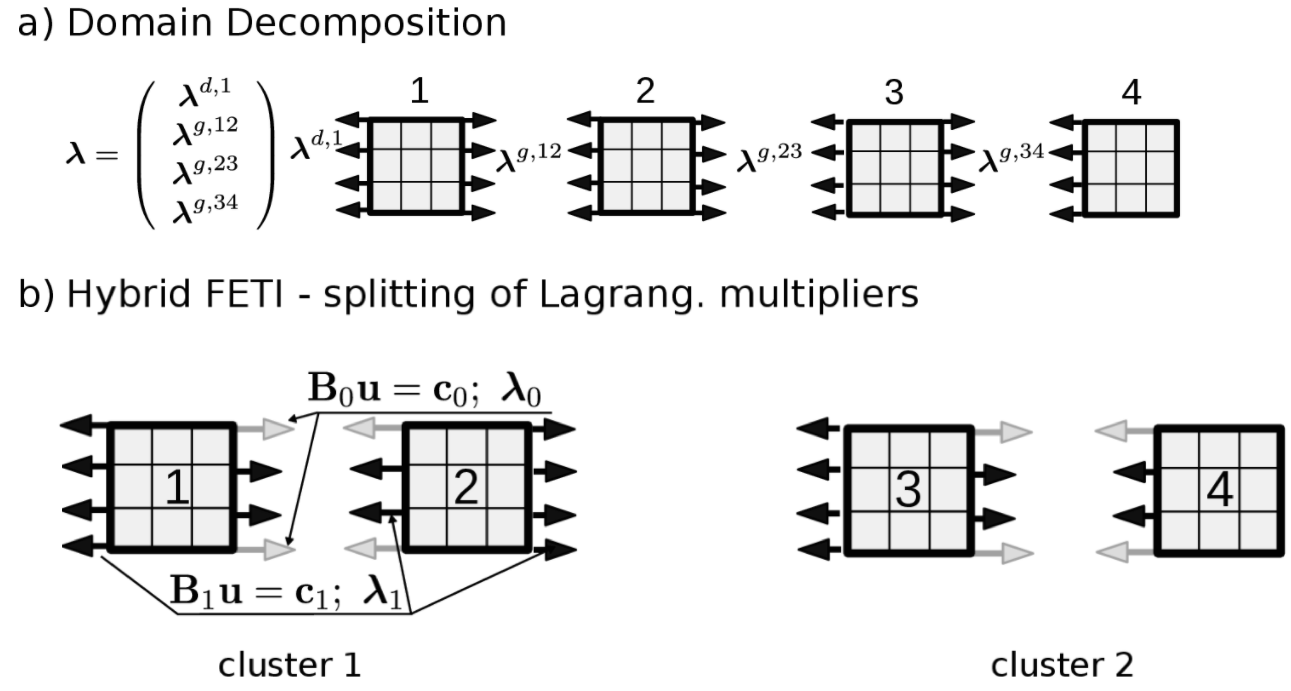
\includegraphics[width=0.9\linewidth]{figures/feti.png}
\end{center}
 \caption{Domain decomposition and splitting of multipliers and cluster formation in FETI.}
 \label{fig:feti}
\end{figure}

Direct solvers are more suitable for smaller problems and iterative solvers are preferred in bigger problems. This solver uses a hybrid approach of using iterative solver and then breaks the problem into sub-problems and applies direct solvers on them. This algorithm ~\cite{feti1, feti2} uses a domain decomposition approach for solving the given linear system for finite element solution in a parallel fashion. The main problem domain is partitioned into non-overlapping sub-domains. These sub-domains are fully-independent, which makes FETI suitable for parallel computing. Each one of these sub-domains is assigned to a separate processor. These sub-domains are connected later on by using Lagrange multipliers on neighboring sub-domains. Each of the sub domain is solved by applying a direct solver to solve the unknowns present in that domain. The solution of the sub-domain problems is then parallelized. This improves the chances of convergence for a given overall. In Figure ~\ref{fig:feti}, the first stage shows the decomposition into four sub-domains and the second stage shows the splitting of Lagrange multipliers and forming clusters. 


\section{Summary}

\begin{figure}[H]
\begin{center}
 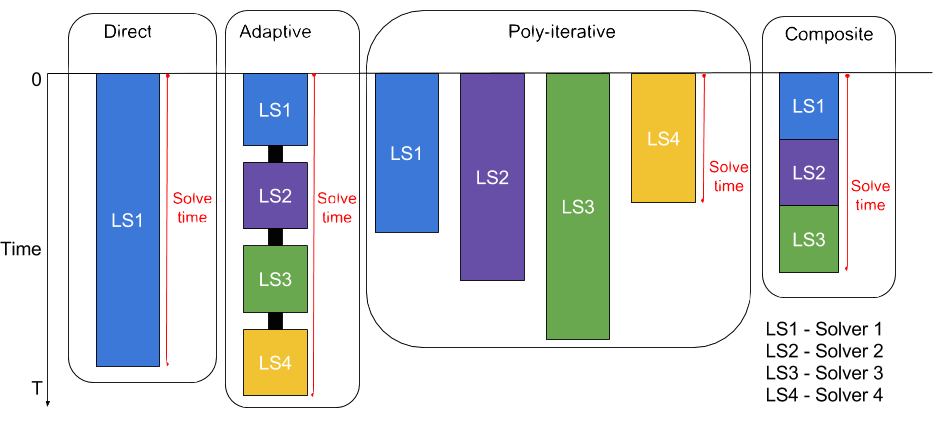
\includegraphics[width=0.95\linewidth]{figures/SolversComparison1.png}
\end{center}
 \caption{Comparison of various solve schemes}
 \label{fig:comparison}
\end{figure}

This chapter presents the two categories of solvers, direct and iterative that can be used for solving large sparse linear systems. Figure~\ref{fig:comparison} shows the various solver techniques discussed in this chapter. Direct solvers use a single solver throughout the process. In an adaptive solver scheme, many solver methods are used although at a time, only one solver is applied. The solver scheme changes the solver based on switching criteria. It runs one solver and then applies the switching check which involves some calculations like convergence rate and increase in the number of iterations. The solver switching is applied multiple times, each time the system decides either to use the same solver or switch to a different solving technique. In poly-iterative approach multiple solvers are applied simultaneously and whichever converges the fastest, terminates the solving process. In the composite solver scheme, the solvers are sequenced in order and everything is preassembled. If the first solver fails, the system switches to the second solver in the order. 


